%!TEX root = ../../report.tex
\chapter{Introduction}

Mobile robot navigation today is highly based on offline generated maps of the environment. 
This is adequate in a lot of applications, but this approach has issues. 
As the discrepancy between the internal map of the robot and the true state of the environment increases, tasks like path planning and localization will be based on more and more erroneous data. 
To overcome these challenges, it would be beneficial to incorporate the dynamics into the representation the robot has of the world.

As the environment changes, a robot which navigation is based on a predetermined static map will be prone to plan paths where there might be placed an obstacle since the map was generated and the time of planning. 
This will force the robot to replan the path thus wasting time or causing the robot to fail to reach its goal. Likewise will a static map based navigation be subject to errors, as the map increasingly misrepresents the environment. 
The most simple solution to these problems would be to add or remove obstacles based on the last observation. This, however, will likely clutter the map with highly dynamical obstacles like people moving through or vehicles driving by and thus has a high risk of blocking large parts of the map. 
Therefore it is necessary to consider which obstacle should be included and which should be left out and furthermore, how this selection is to be done.

\section{Aims}
This thesis aims to solve the task of representing the world as it changes, in order to uphold a useful representation for navigation and localization purposes. 
The solution should be based on commonly used, on-board sensors thus not requiring additional infrastructure to be established in the area of operation. 
It is chosen to make the solution easily integratable with existing systems, requiring no hardware changes. 
In order to maintain an up-to-date representation of the world it is necessary to determine an effective way of representing the changes and to continuously learn the dynamics of the environment. 
The learning must be able to account for changes in the dynamics. 
This is due to the fact that it can not be expected for the dynamics to remain on the same level throughout time. The method must be able to cope with both the differentiating between static and dynamics and changes in the level of dynamics in an area. 
As various sources of noise are expected in a real world scenario, these should be integrated into the learning system to provide a better basis for learning. One of the sources that should be considered is the sensor noise, which could degrade the perception of the environment. Another is the localisation noise.
As the system should run without extra infrastructure, whatever localisation uncertainty is within any onboard localisation system used, this should be taken into account.
In learning the dynamics it is also necessary to convert the learned dynamics into a usable map for navigation and localisation systems. Rules for this conversion will have to take into account the desired types of obstacles to be represented. 
A user might want to only represent static obstacles, for instance walls and heavy machinery, for localization purposes but also more dynamic obstacles when path planning and navigating. 
As this could vary between users and application it could be beneficial to add this as one of the inevitable parameters necessary to tune the final method for specific uses. 

Summing up, this project strives to improve navigation with mobile robots through continuous learning of the dynamic environment with onboard sensors. Specifically the following problems are considered:

\begin{itemize}
\item Long-term fast adaptive map representation of dynamic environments
\item Precise mapping of static environment by incorporation of sensor and localization noise
\item Learning dynamics in environments
\item Full scale evaluation on the MIR100 platform
\end{itemize}

\section{Thesis core}
The system that has been devised in order to achieve the above mentioned goals can be considered in three main sections; static mapper, dynamic learner and interpretation. 
Figure \ref{fig:block-overview} shows an overview of the sections and their connections. 
The static mapper handles the sensor input. This is used to build up a momentary image of the environment. It is in this section the noise is integrated and accounted for. 
These momentary maps are provided to the dynamics learner which uses them to learn the dynamics of the world. 
The learner maintains an internal representation of the dynamics of the environment. 
In order to provide a useful output for the navigation and localization systems the interpretation sections handles the conversion from the internal dynamic environment representation. 

\begin{figure} [htbp]
	\centering
	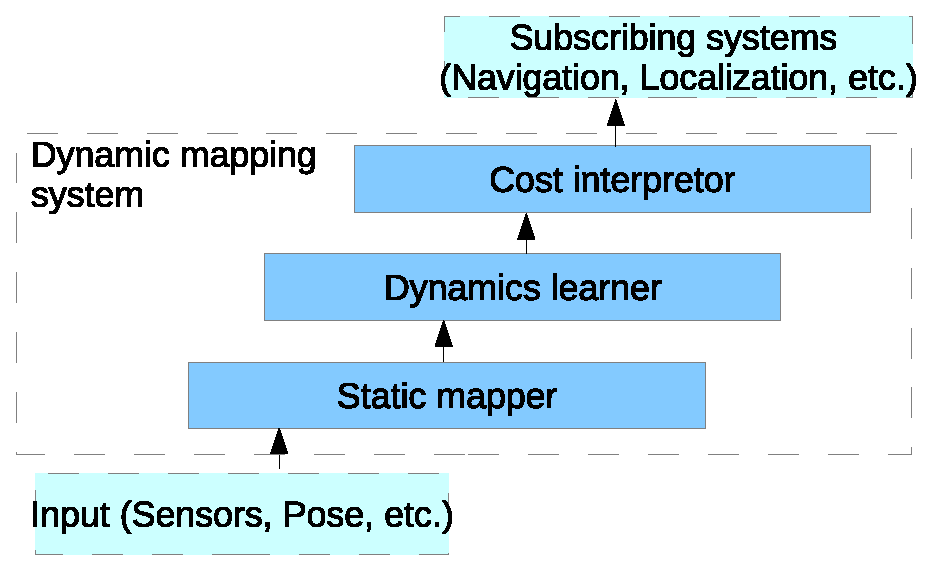
\includegraphics[scale=0.7]{chapters/introduction/figures/system-overview}
	\caption{Block overview of the dynamic mapping system}
	\label{fig:block-overview}
\end{figure}

\subsection{Thesis outline}

New stuff\\
Long term navigation dynamic environment
- Wrong / suboptimal path planning
- Failed localization

Requirements
Plasticity
- Adapt quickly to changes 
- Avoid insertion errors -> recursion problem (localization on updated map -> new map based on localization)
- Avoid bad landmarks

Pre- assumption
2D world
Lidar sensor only
Preferably an easy interface 
Changes in the environment are continuos and partial. Areas are visited more frequently than significant changes. (change per visit?)

It should be able to run online
Nice: low resource requirements




